\documentclass[Calculus 1 Recitation.tex]{subfiles}

\begin{document}
\section{Applications of Differentiation}
\subsection{Maximum and Minimum Values}
\begin{myleftlinebox}
	global maximum/minimum, extreme values
	\tcblower
	Let $c\in D$, the domain of $f$. Then $f(c)$ is the
	\begin{itemize}
		\item global maximum, or absolute maximum, value of $f$ on $D$, if $f(c)\geq f(x)$, $\forall x\in D$.
		\item global minimum, or absolute minimum, value of $f$ on $D$, if $f(c)\leq f(x)$, $\forall x\in D$.
	\end{itemize}
	They are the extreme values of $f$.
\end{myleftlinebox}

\begin{myleftlinebox}
	local maximum/minimum
	\tcblower
	Let the neighborhood of $c$ is in $D$, the domain of $f$. Then $f(c)$ is the
	\begin{itemize}
		\item local maximum value of $f$, if $f(c)\geq f(x)$, when $x$ is near $c$
		\item local minimum value of $f$, if $f(c)\leq f(x)$, when $x$ is near $c$
	\end{itemize}
	Here being true "near" $c$ means being true on some open interval containing $c$.
\end{myleftlinebox}

\begin{myleftlinebox}
	The Extreme Value Theorem
	\tcblower
	\begin{theorem}
		If $f$ is continuous on a closed interval $[a,b]$, then $f$ attains an absolute maximum value at $f(c)$ and an absolute minimum value $f(d)$ at some $c,d\in[a,b]$.
	\end{theorem}
\end{myleftlinebox}

\begin{myleftlinebox}
	critical number
	\tcblower
	A critical number of $f$ is a number $c$ in the domain $D$ such that either $f'(c)=0$ or $f'(c)$ doesn't exist.
\end{myleftlinebox}

\begin{myleftlinebox}
	The Fermat's Theorem
	\tcblower
	\begin{theorem}
		If $f$ has a local maximum or minimum at $c$, and if $f'(c)$ exists, then $f'(c)=0$. In terms of critical numbers, $c$ is a critical number of $f$.
	\end{theorem}
\end{myleftlinebox}

\begin{myleftlinebox}
	closed interval method
	\tcblower
	To find the absolute maximum/minimum value of a function $f$ on a closed interval $[a,b]$,
	\begin{enumerate}
		\item find the values of $f$ at the critical numbers of $f$ in $(a,b)$
		\item find the values of $f$ at the endpoints of the interval
		\item the largest of the values from step 1 and 2 is the absolute maximum value, and the smallest of these values is the absolute minimum value.
	\end{enumerate}
\end{myleftlinebox}

\subsection{The Mean Value Theorem}

\begin{myleftlinebox}
	Rolle's Theorem
	\tcblower
	\begin{theorem}
		Let $f$ be a function that satisfies the following three conditions:
		\begin{itemize}
			\item $f$ is continuous on $[a,b]$
			\item $f$ is differentiable on $(a,b)$
			\item $f(a)=f(b)$
		\end{itemize}
		then $\exists c\in(a,b)$ such that $f'(c)=0$.
	\end{theorem}
\end{myleftlinebox}

\begin{myleftlinebox}
	The Mean Value Theorem
	\tcblower
	\begin{theorem}
		Let $f$ be a function that satisfies the following two conditions:
		\begin{itemize}
			\item $f$ is continuous on $[a,b]$
			\item $f$ is differentiable on $(a,b)$
		\end{itemize}
		then $\exists c\in(a,b)$ such that $f'(c)=\frac{f(b)-f(a)}{b-a}$.
	\end{theorem}
\end{myleftlinebox}

\begin{myleftlinebox}
	some facts
	\tcblower
	\begin{proposition}
		If $f'(x)=0$ for all $x\in(a,b)$, then $f$ is a constant on $(a,b)$. And if $f'(x)=g'(x)$ for all $x\in(a,b)$, then $f=g+c$ on $(a,b)$ where $c$ is a constant.
	\end{proposition}
\end{myleftlinebox}

\subsection{What Derivatives Tell Us about the Shape of a Graph}

\begin{myleftlinebox}
	increasing, decreasing test
	\tcblower
	\begin{itemize}
		\item if $f'(x)>0$ on an interval, then $f$ is increasing on that interval
		\item if $f'(x)<0$ on an interval, then $f$ is decreasing on that interval
	\end{itemize}
\end{myleftlinebox}

\begin{myleftlinebox}
	first derivative test
	\tcblower
	\begin{itemize}
		\item if $f'(x)$ changes from positive to negative at $a$, then $f$ has a local maximum at $a$
		\item if $f'(x)$ changes from negative to positive at $a$, then $f$ has a local minimum at $a$
		\item otherwise $f$ has no local maximum or minimum at $a$
	\end{itemize}
\end{myleftlinebox}

\begin{myleftlinebox}
	concave upward and downward
	\tcblower
	If the graph of $f$ lies above all its tangents on an interval $I$, then $f$ is concave upward on $I$. If the graph of $f$ lies below all its tangents on an interval $I$, then $f$ is concave downward on $I$.
\end{myleftlinebox}

\begin{myleftlinebox}
	concavity test
	\tcblower
	\begin{itemize}
		\item if $f''(x)>0$ on an interval, then $f$ is concave upward on that interval
		\item if $f''(x)<0$ on an interval, then $f$ is concave downward on that interval
	\end{itemize}
\end{myleftlinebox}

\begin{myleftlinebox}
	inflection point
	\tcblower
	A point $P$ on a curve $y = f(x)$ is called an inflection point if $f$ is continuous there and the curve changes from concave upward to concave downward.
\end{myleftlinebox}

\begin{myleftlinebox}
	first derivative test
	\tcblower
	\begin{itemize}
		\item if $f'(a)=0$ and $f''(a) > 0$, then $f$ has a local minimum at $a$
		\item if $f'(a)=0$ and $f''(a) < 0$, then $f$ has a local maximum at $a$
	\end{itemize}
\end{myleftlinebox}

\subsection{Limits at Infinity; Horizontal Asymptotes}

\begin{myleftlinebox}
	limit at infinity
	\tcblower
	We use the notation $\lim_{x\to\infty} f(x)=L$. Let $f$ be a function defined on some interval $(a,\infty)$, then limit of $f$ at positive infinity is $L$ if values of $f$ can be made arbitrarily close to $L$ by requiring $x$ to be sufficiently large.\\
	In $\epsilon-\delta$ language, $\forall \epsilon >0$, $\exists M>0$ such that $\forall x>M$, $\abs{f(x)-L}<\epsilon$.\\
	Limit at negative infinity can be defined similarly.
\end{myleftlinebox}

\begin{myleftlinebox}
	horizontal asymptote
	\tcblower
	Line $y=L$ is a horizontal asymptote of function $y=f(x)$ if either $\lim_{x\to\infty} f(x)=L$ of $\lim_{x\to-\infty} f(x)=L$
\end{myleftlinebox}

\begin{myleftlinebox}
	limit of negative rational power function at infinity
	\tcblower
	\begin{theorem}
		if $r$ is a rational number, then $\lim_{x\to\infty} \frac{1}{x^r}=0$. Further if $x^{r}$ is defined for all $x$, then $\lim_{x\to-\infty} \frac{1}{x^r}=0$.
	\end{theorem}
\end{myleftlinebox}

\begin{myleftlinebox}
	infinity limits at infinity
	\tcblower
	Notation $\lim_{x\to\infty} f(x)=\infty$ is used to indicates that the values of $f(x)$ become infinitely large as $x$ goes to infinity.\\
	In $\epsilon-\delta$ language, $\forall M >0$, $\exists x(M)>0$ such that $\forall x>x(M)$, $f(x)>M$.
\end{myleftlinebox}

\subsection{Summary of Curve Sketching}
\begin{myleftlinebox}
	guidelines for plotting $y=f(x)$
	\tcblower
	\begin{enumerate}
		\item domain and plot range: select where to plot the function so that the interesting parts are included
		\item intercepts: mark $f(0)$ on $y$-axis and roots for $f(x)=0$ on $x$-axis if possible
		\item symmetry: check if $f$ is odd or even, or can be shifted or stretched to an odd or even function $g$, and also check if the function is periodic or not
		\item asymptotes: use dashed line to plot horizontal asymptotes and vertical asymptotes. Slant asymptotes and other higher order asymptotes will be discussed later
		\item intervals of increase and decrease: calculate $f'(x)$ and check its positivity
		\item local maximum or minimum: solve $f'(x)=0$ and check if $f''(x)\neq 0$
		\item concavity and points of inflection: calculate $f''(x)$ and check its positivity
	\end{enumerate}
\end{myleftlinebox}

\begin{myleftlinebox}
	slant asymptote
	\tcblower
	If $\lim_{x\to\infty} f(x)-(kx+b)=0$ or $\lim_{x\to-\infty} f(x)-(kx+b)=0$, then line $y=kx+b$ is a slant asymptote for $f(x)$.
\end{myleftlinebox}

\subsection{Graphing with Calculus and Technology}
\begin{myleftlinebox}
	some ready-to-use graphing tools
	\tcblower
	\begin{itemize}
		\item graphing calculator: \href{https://www.amazon.com/s?k=graphing+calculator}{link to Amazon}
		\item \href{https://www.desmos.com/calculator}{Desmos}
		\item \href{https://www.mathway.com/Graph}{Mathway}
		\item \href{https://www.geogebra.org/graphing}{Geogebra}
		\item \href{https://www.symbolab.com/graphing-calculator}{Symbolab}
		\item \href{https://www.wolframalpha.com/}{Wolframalpha}
	\end{itemize}
\end{myleftlinebox}

\begin{myleftlinebox}
	some graphing tools with coding
	\tcblower
	\begin{itemize}
		\item Python with matplotlib
		\item R with ggplot2
		\item Wolfram Mathematica
		\item MATLAB and GNU Octave 
		\item TikZ and PGF in \LaTeX
		\item Julia with Plots
		\item C++ with sciplot or matplotlib
	\end{itemize}
\end{myleftlinebox}

\subsection{Optimization Problems}
\begin{myleftlinebox}
	first derivative test for absolute extreme values
	\tcblower
	\begin{itemize}
		\item if $f'(x)>0$ for all $x<c$ and $f'(x)<0$ for all $x>c$, then $f(c)$ is the absolute maximum value of $f$
		\item if $f'(x)<0$ for all $x<c$ and $f'(x)>0$ for all $x>c$, then $f(c)$ is the absolute minimum value of $f$
	\end{itemize}
\end{myleftlinebox}

\begin{myleftlinebox}
	some definitions from business and economics literature
	\tcblower
	Case: a company is producing and selling a product
	\begin{itemize}
		\item cost function: $C(x)$ where $x$ is the number of unit produced and $C(x)$ is the cost for producing $x$ units
		\item marginal cost: $C'(x)$
		\item demand function/price function: $p(x)$ is the price per unit if the company sells $x$ unit
		\item revenue function: $R(x)=xp(x)$
		\item marginal revenue function: $R'(x)$
		\item profit function: $P(x)=R(x)-C(x)$
		\item marginal profit function: $P'(x)$
	\end{itemize}
\end{myleftlinebox}

\subsection{Newton's Method}
\begin{myleftlinebox}
	Newton's Method
	\tcblower
	An algorithm to find a root of a real-valued function.
	\begin{enumerate}
		\item prepare a staring point $x_0$
		\item let $x_{i+1}=x_i-\frac{f(x_i)}{f'(x_i)}$
		\item keep doing step 2 until $|x_{n+1}-x_n|<\epsilon$ where $\epsilon$ is the error tolerance
	\end{enumerate}
	\begin{remark}
		this basic version of Newton's Method would fail for various reasons. Another basic root-finding algorithm is bisection method.
	\end{remark}
\end{myleftlinebox}

\subsection{Antiderivatives}
\begin{myleftlinebox}
	antiderivative
	\tcblower
	A function $F$ is called the antiderivative of $f$ on an interval $I$ if $F'(x)=f(x)$ for all $x\in I$.
	\begin{theorem}
		If $F$ is an antiderivative of $f$ on an interval $I$, then the most general antiderivative of $f$ on $I$ is $F(x)+C$ where $C$ is an arbitrary constant.
	\end{theorem}
\end{myleftlinebox}

\begin{myleftlinebox}
	antidifferentiation formulas
	\tcblower
	\begin{center}
		\begin{tabular}{cc|cc}
			\hline
			Function & Particular antiderivative & Function & Particular antiderivative\\\hline
			$cf(x)$ & $cF(x)$ & $\cos(x)$ & $\sin(x)$\\
			$f(x)+g(x)$ & $F(x)+G(x)$ & $\sin(x)$ & $-\cos(x)$\\
			$x^n$, $n\neq 1$ & $\frac{x^{n+1}}{n+1}$ & $\frac{1}{\cos^2(x)}$ & $\tan(x)$\\
			\hline
		\end{tabular}
	\end{center}
\end{myleftlinebox}

\subsection{Exercises}

\begin{myleftlinebox}
	find the global/local maximum/minimum of function: $x^3-3x^2+6$ on interval $[-1,2]$.
	\tcblower
	\vspace{2em}	
\end{myleftlinebox}

\begin{myleftlinebox}
	find the critical numbers of functions: $x+1/x$, $\tan(x)$, $x\sin(6x^2)$.
	\tcblower
	\vspace{2em}	
\end{myleftlinebox}

\begin{myleftlinebox}
	Assume $0<\alpha<\beta<\pi/2$, prove 
	\[\frac{\beta-\alpha}{\cos^2\alpha}<\tan\beta-\tan\alpha<\frac{\beta-\alpha}{\cos^2\beta}\]
	\tcblower
	\vspace{2em}	
\end{myleftlinebox}

\begin{myleftlinebox}
	Prove $\abs{\sin x-\sin y} \leq \abs{x-y}$, $x,y\in\bR$
	\tcblower
	\vspace{2em}	
\end{myleftlinebox}

\begin{myleftlinebox}
	Prove Cauchy's Mean Value Theorem. 
	\begin{theorem}
		Let $f,g$ be two functions that satisfy the following three conditions:
		\begin{itemize}
			\item $f,g$ is continuous on $[a,b]$
			\item $f,g$ is differentiable on $(a,b)$
			\item $g'\neq0$ when $x\in(a,b)$
		\end{itemize}
		then $\exists c\in(a,b)$ such that $\frac{f(b)-f(a)}{g(b)-g(a)}=\frac{f'(c)}{g'(c)}$.
	\end{theorem}
	\tcblower
	\vspace{2em}	
\end{myleftlinebox}

\begin{myleftlinebox}
	Assuming $f$ is differentiable at $[0,\infty)$ and $0\leq f(x)\leq \frac{x}{1+x^2}$, prove there exists a $c>0$ such that
	\[f'(c)=\frac{1-c^2}{(1+c^2)^2}\]
	\tcblower
	\vspace{2em}
\end{myleftlinebox}

\begin{myleftlinebox}
	If $f'(x)\neq 1$ for all real numbers $x$, then $f(x)=x$ has at most one solution.
	\tcblower
	\vspace{2em}
\end{myleftlinebox}

\begin{myleftlinebox}
	Use two methods to prove there's exactly one solution to the equation $3x=\sin(x)$. The first is some mean value theorem, and the second is based on derivatives.
	\tcblower
	\vspace{2em}	
\end{myleftlinebox}

\begin{myleftlinebox}
	Let $f(x)=x+\frac{1}{x}$. Find the intervals where it's increasing, where it's decreasing, where it's concave upward and where it's concave downward.
	\tcblower
	\vspace{2em}
\end{myleftlinebox}

\begin{myleftlinebox}
	Let $f(x)=\sin(x)$. Find the intervals where it's increasing, where it's decreasing, where it's concave upward and where it's concave downward. Then find all its inflection points.
	\tcblower
	\vspace{2em}
\end{myleftlinebox}

\begin{myleftlinebox}
	Show that the inflection points of the curve $y=x\cos (x)$ lie on the curve $y^2(x^2+4)=4x^2$.
	\tcblower
	\vspace{2em}	
\end{myleftlinebox}

\begin{myleftlinebox}
	Show that the inflection points of the curve $y=\frac{1+x}{1+x^2}$ lies on the same straight line.
	\tcblower
	\vspace{2em}	
\end{myleftlinebox}

\begin{myleftlinebox}
	Find the set for value $c$ such that function $f(x)=cx+\frac{1}{x^2+1}$ is increasing on $(-\infty,\infty)$.
	\tcblower
	\vspace{2em}	
\end{myleftlinebox}

\begin{myleftlinebox}
	Use $\epsilon-\delta$ language to say that $\sin(x)$ doesn't have limit at infinity.
	\tcblower
	\vspace{2em}
\end{myleftlinebox}

\begin{myleftlinebox}
	Sketch the following functions: $y=(x-5)^2+3$, $y=(x-1)(x-2)(x-3)$, $y=x^2(x-6)$. Then find their critical points and categorize them as a local maximum, a local minimum, or neither.
	\tcblower
	\vspace{2em}
\end{myleftlinebox}

\begin{myleftlinebox}
	For what values of $c$ is there a straight line that intersects the following curve in four distinct points?
	\[y=x^4+cx^3+x^2+x+1\]
	\tcblower
	\vspace{2em}
\end{myleftlinebox}

\begin{myleftlinebox}
	Calculate the following limit where $a_n,b_n\neq 0$.
	\[\lim_{x\to\infty}\frac{a_n x^n}{b_n x^n}, \lim_{x\to\infty}\frac{a_n x^n+a_{n-1} x^{n-1}}{b_n x^n+b_{n-1} x^{n-1}}\]
	\tcblower
	\vspace{2em}
\end{myleftlinebox}

\begin{myleftlinebox}
	Calculate the asymptote of 
	\[\frac{a_3 x^3+a_2 x^2+a_1 x+a_0}{b_1 x+b_0}\]
	, where $a_3,b_1\neq0$. And you can put any numbers you like as coefficients.
	\tcblower
	\vspace{2em}
\end{myleftlinebox}

\begin{myleftlinebox}
	Show that $x^2(4-x^2)\leq 4$ for all numbers $x$ such that $|x|\leq 2$.
	\tcblower
	\vspace{2em}
\end{myleftlinebox}

\begin{myleftlinebox}
	Consider a semi-ellipse above the $x$-axis with expression: $\frac{x^2}{a^2}+\frac{y^2}{b^2}=1$, $y\geq 0$. Find the area of the largest rectangle that can be inscribed inside.
	\tcblower
	\vspace{2em}
\end{myleftlinebox}

\begin{myleftlinebox}
	Find the point on the parabola $y=6x^2$ that is closest to the point $(3,3)$.
	\tcblower
	\vspace{2em}
\end{myleftlinebox}

\begin{myleftlinebox}
	A cylinder container with an open top is to be constructed from a square piece of cardboard, 3 ft wide. Find the largest volume that such a container can have.
	\tcblower
	\vspace{2em}
\end{myleftlinebox}

\begin{myleftlinebox}
	Find the general antiderivatives of the following functions: $f(x)=\frac{1+t}{t^2}$, $g(x)=\sin(x)+\pi\cos(x)$.
	\tcblower
	\vspace{2em}
\end{myleftlinebox}

\begin{myleftlinebox}
	Show that for motion in a straight line with constant acceleration $a$, initial velocity $v_0$, and initial displacement $s_0$, the displacement after time is $s=\frac{1}{2}at^2+v_0t+s_0$.
	\tcblower
	\vspace{2em}
\end{myleftlinebox}

\newpage

\subsection{Practice Exam}

\begin{myleftlinebox}
	Find all the asymptotes for the following function.
	\begin{center}
		%ref: https://vincenttam.gitlab.io/page/tikz-templates/
		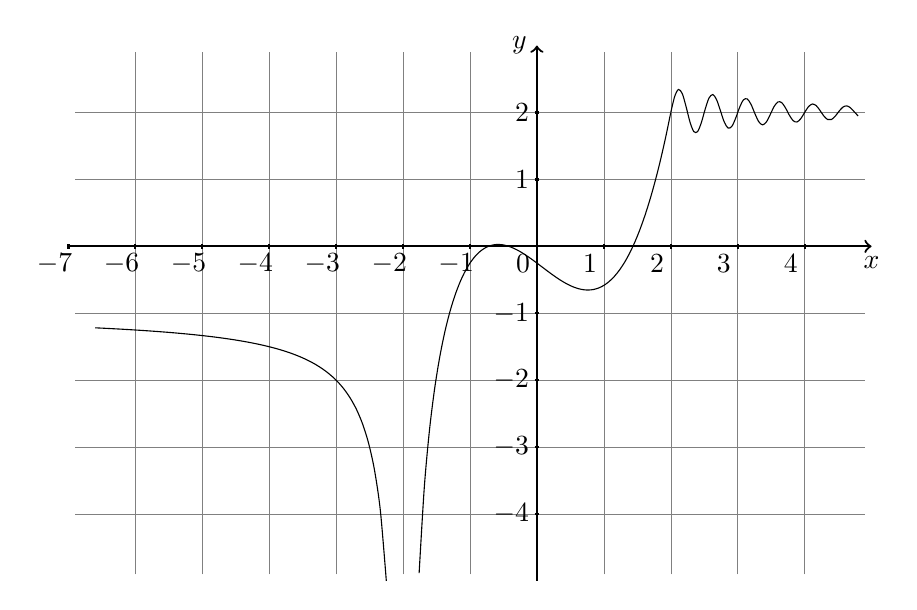
\begin{tikzpicture}[scale=0.850]
			\draw[help lines,step=1 cm](-6.9,-4.9) grid (4.9,2.9);
	
			% x-axis
			\draw [thick] [->] (-7,0)--(5,0) node[right, below] {$x$};
			\foreach \x in {-7,...,4}
			\draw[xshift=\x cm, thick] (0pt,-1pt)--(0pt,1pt) node[xshift=-5pt, yshift=-7pt] {$\x$};
	
			% y-axis
			\draw [thick] [->] (0,-5)--(0,3) node[above, left] {$y$};
			\foreach \y in {-4,-3,-2,-1,1,2}
			\draw[yshift=\y cm, thick] (-1pt,0pt)--(1pt,0pt) node[left] {$\y$};
	
			% function plot(s)
			\draw [domain=2:4.8, variable=\x, samples=50, smooth]
			plot ({\x}, {sin(\x*720)/(exp(0.5*\x))+2});

			\draw [domain=-1.76:2, variable=\x, samples=50, smooth]
			plot ({\x}, {-1/(\x+2)+\x*\x*\x/2-\x+0.25});

			\draw [domain=-6.6:-2.25, variable=\x, samples=50, smooth]
			plot ({\x}, {1/(\x+2)-1});
		\end{tikzpicture}
	\end{center}
	\tcblower
\end{myleftlinebox}

\begin{myleftlinebox}
	Sketch a graph of $f(x)$ that is continuous and differentiable on the domain $(-\infty,0)\cup (0,\infty)$ that satisfies the following conditions. (and some bonus points if you can specify one)
	\begin{itemize}
		\item $f(-1)=f(1)=f(3)=0$
		\item $\displaystyle \lim_{x\to-\infty}f(x)=0, \lim_{x\to+\infty}f(x)=-\infty$
		\item $\displaystyle \lim_{x\to 0^-}f(x)=+\infty, \lim_{x\to 0^+}f(x)=-\infty$
		\item $f'(-2)=f'(2)=0$
		\item $f'(x)>0$ if $-1<x<0$ or $0<x<2$
		\item $f'(x)<0$ if $x<-1$ or $2<x$
		\item $f''(-3)=0$
		\item $f''(x)>0$ if $-3<x<0$
		\item $f''(x)<0$ if $x<-3$ or $x>0$
	\end{itemize}
	\tcblower
\end{myleftlinebox}

\begin{myleftlinebox}
	Pick a point $(x,y)$ on function $f(x)=\frac{1}{1+(x+2)^2}$ to maximize $xy$.
	\tcblower
\end{myleftlinebox}

\begin{myleftlinebox}
	(Chapter 3 Problem Plus 24) A hemispherical bubble is placed on a spherical bubble of radius 1. A smaller hemispherical bubble is then placed on the first one. This process is continued until n chambers, including the sphere, are formed. Use mathematical induction to prove that the maximum height of any bubble tower with n chambers is $1+\sqrt{n}$.
	\tcblower
\end{myleftlinebox}

\begin{myleftlinebox}
	Find function $f(x)$ with $f'(x)=3x^2+2x+1$ and the line $y=x$ is tangent to the graph of $f$.
	\tcblower
\end{myleftlinebox}

\end{document}